\documentclass[letterpaper,12pt]{article}
\usepackage[utf8]{inputenc}
\usepackage{amsmath}
\usepackage{amsfonts}
\usepackage{amssymb}
\usepackage{enumerate}
\usepackage[margin=0.75 in]{geometry}
\usepackage{graphicx}

\newcommand{\aaa}{\mathbf{a}}
\newcommand{\bbb}{\mathbf{b}}
\newcommand{\abs}[1]{\lvert #1\rvert}
\newcommand{\len}[1]{\lVert #1\rVert}
\newcommand{\dotp}{\boldsymbol{\cdot}}
\renewcommand{\r}{\mathbf{r}}
\newcommand{\x}{\mathbf{x}}
\newcommand{\R}{\mathbb{R}}
\newcommand{\di}{\displaystyle}
%opening
\title{On parametric curves and area}
\author{Sean Fitzpatrick}

\begin{document}

\maketitle
\section{Parametric curves}
Since we weren't able to spend much time discussing area for parametric and polar curves, I've prepared this handout to highlight some of the main points (especially those neglected in Stewart). First, let's recall that a parametric curve in $\R^2$ is given by a continuous map
\[
 F:I\subseteq\R \to \R^2;\quad F(t) = (x(t),y(t)),
\]
which we sometimes express in terms of the corresponding vector-valued function $\r(t) = \langle x(t),y(t)\rangle$. Here $I\subseteq \R$ is an interval, which is usually a closed interval $[a,b]$. Note that continuity in this case means that for any $\epsilon>0$, there exists a $\delta>0$ such that $0<\abs{t-t_0}<\delta$ implies $\sqrt{(x(t)-x(t_0))^2+(y(t)-y(t_0))^2} = \len{\r(t)-\r(t_0)}<\epsilon$. (Recall, from an earlier assignment problem, that this is equivalent to the continuity of the component functions $x(t)$ and $y(t)$.) 

A parametric curve $F:[a,b]\to\R^2$ is {\bf smooth} if corresponding vector-valued function $\r(t)$ is continuously differentiable on $(a,b)$; that is, if the tangent vector $\r'(t) = \langle x'(t),y'(t)\rangle$ is defined and continuous on $(a,b)$, and $\r'(t)\neq 0$ for all $t\in (a,b)$. Any parametric curve defined on an interval $[a,b]$ has an {\em orientation} induced by the usual left-to-right orientation of the real line: we think of $F(a)$ as the {\em initial point} of the curve, and $F(b)$ as the {\em final point}. A {\em reparametrization} of $F$ is given by a function $h:[c,d]\to [a,b]$, where $h'(u)\neq 0$ for all $u\in (c,d)$. With $t=h(u)$ we define $G:[c,d]\to\R^2$ by
\[
 G(u) = F(h(u))=F(t).
\]
Notice that this implies that the images of $F$ and $G$ in $\R^2$ are the same: $F$ and $G$ are different {\em parametric} curves, but the resulting curve in $\R^2$ is the same. If $h'(u)>0$, $F$ and $G$ have the same orientation, but if $h'(u)<0$, then $F$ and $G$ have opposite orientations. 
\subsection{Arc length}
The notion of reparameterization is important for understanding the arc length formula for a parametric curve. Given a parametric curve $F:[a,b]\to\R^2$, we defined the length of the curve defined by $F$ to be
\[
 L = \int_a^b\len{\r'(t)}\,dt.
\]
There are two issues to be mindful of here. One is that we need to make sure that our parametric curve doesn't trace out a given curve more than once --- we want to compute the length of a curve, not the total distance travelled along it. This can be dealt with by requiring that $F$ be a one-to-one function (with the exception of $F(a)=F(b)$ for closed curves, as well as some finite number of self-intersections). If $F$ is not a closed curve, this follows from the requirement that $\r'(t)\neq 0$. (In order to pass by the same point twice, you'd have to turn around, and in order to reverse direction, you have to stop.) For closed curves one has to be more careful. For example, the curve $F(t)=(\cos 4t, \sin 4t)$, with $t\in [0,2\pi]$, goes around the unit circle four times without stopping. 

The second issue is to make sure that the ``speed'' at which the curve is travelled doesn't affect the integral; that is, that the arc length does not depend on a choice of parametrization. At first, it seems like the speed should matter: after all, we compute the length by integrating $\len{\r'(t)}$, which is precisely the speed! However, when we change the speed, we also change the ``time of travel'' (the length of the integral). If $G(u)$ is a reparametrization of $F(t)$ (that is, $t=h(u)$ for some function $h$), we have the corresponding vector-valued functions $\r_G(u) = \r_F(h(u))$, and the chain rule gives us
\[
 \len{\r_G'(u)} = \len{\r_F'(h(u))}\abs{h'(u)}.
\]
Thus, we find that (assuming $h'(u)>0$)
\[
 \int_a^b\len{\r_F'(t)}\,dt = \int_c^d\len{\r_F'(h(u))}h'(u)\,du = \int_c^d\len{\r_G'(u)}\, du.
\]
The integral on the left is what we'd compute if we started with $F$, and the integral on the right is what we'd compute if we started with $G$, and we see that they're equal by the usual substitution rule. (If $h'(u)<0$, the limits of integration get swapped, but we also have $\abs{h'(u)}=-h'(u)$, and the minus sign swaps the limits back, giving the same result.)
\subsection{Area}
Let us now return to the problem of finding area. Suppose we have a graph $y=f(x)$ parametrized by $F(t) = (x(t),f(x(t)))$ for $t\in [a,b]$. In class, we derived the formula $\di A=\int_a^b y(t)x'(t)\,dt$ from the ``area under the curve'' result in single-variable calculus: $\di A = \int_c^d f(x)\,dx$, where $y=f(x)$ and if $x=x(t)$, we get $dx = x'(t)\,dt$, $y(t) = f(x(t))$. 

There is one catch, however: \emph{this formula is only valid if $x'(t)>0$}. The usual area formula assumes that we work from left to right, in the direction of increasing $x$. If we parametrize the curve so that it is traced out from right to left, our area will be negative, and we need a minus sign in front to compensate.

The area formula for parametric curves is more versatile than simple area under a graph, however: it can be used to compute areas defined by parametric curves that are {\em not} the graph of a function. In other words, given $F(t)=(x(t),y(t))$ we can't eliminate the parameter $t$ using a function $f$ such that $y=f(x)$ --- the circle again provides a good example here. Usually this situation arises when our curve has one or more vertical tangents, where $x'(t)=0$.\\ ({\em Exercise}: prove that if $x'(t)\neq 0$ for all $t$, then it {\em is} possible to solve for $y$ as a function of $x$.)

In order to define an area, we need to deal with {\em closed} curves, where $F(a)=F(b)$. When this is not the case, the convention is to revert to the ``area under the curve'' picture from single-variable calculus. To avoid ambiguity we usually require that our curves be {\em simple}, meaning that there are no self-intersections, as illustrated below:
\begin{center}
 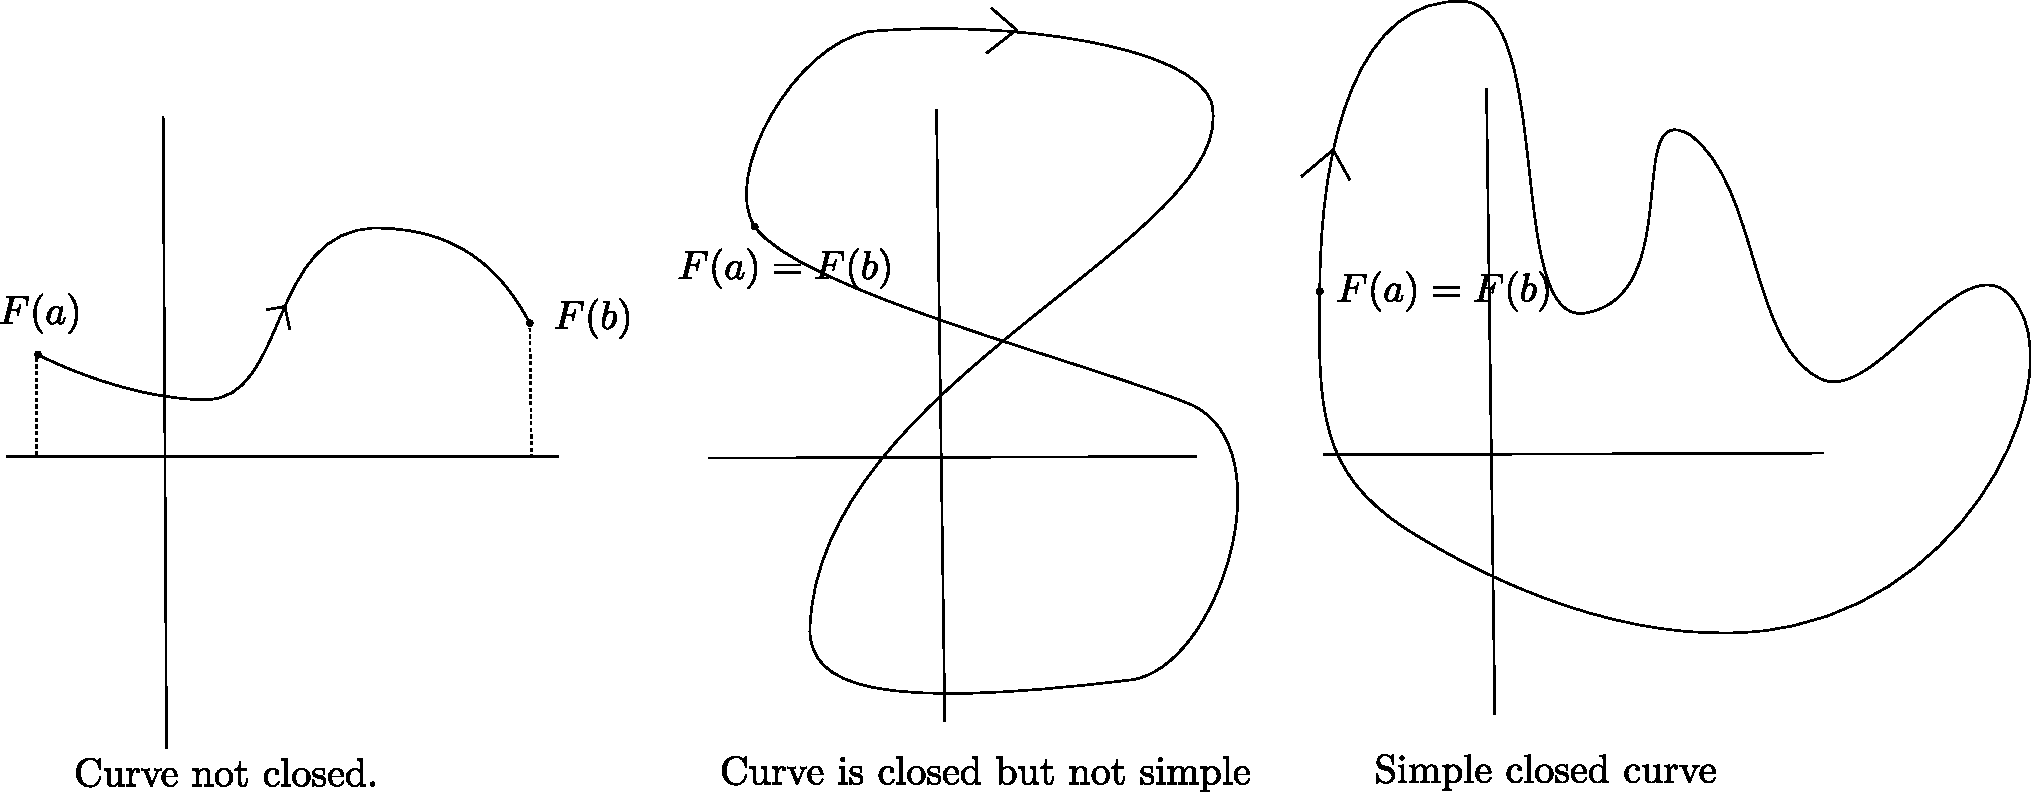
\includegraphics[width=5in]{Curves.pdf}
\end{center}
Note that in the latter case, there is a clearly-defined area. This is the situation in which the parametric area formula is most useful. However, since we derived this formula from the rule for calculating area under a curve (like on the left in the above image), we need to ensure that it is still the case that $\di A = \int_a^b y(t)x'(t)\,dt$ for any simple closed piecewise-smooth curve.
In fact, this formula is not quite right. Parametric curves are oriented, and changing this orientation changes the sign of the integral computing the area. For closed curves, the convention is that a {\em positively-oriented curve} is one with a counter-clockwise orientation. (If you imagine yourself walking along the curve, you are walking in the positively-oriented direction if the area to be computed is on your left.) With this convention, the correct area formula is
\[
 A = -\int_a^b y(t)x'(t)\,dt.
\]
 Feel free to check this on some easy examples, like the circle. Now, why is it valid? Often students are most concerned about the case where the curve lies both above and below the $x$-axis. However, it's easy to see that translating the curve has no effect on the area: if we replace $y(t)$ by $y(t)+C$ for some constant $C$, then
\[
 -\int_a^b (y(t)+C)x'(t)\,dt = -\int_a^by(t)x'(t)\,dt -\int_a^b Cx'(t)\,dt = A -C(x(b)-x(a)) = A,
\]
since $x(a)=x(b)$ for closed curves. So if our curve did lie partly below the $x$-axis, we could simply add a sufficiently large constant to $y(t)$ to shift the entire thing about the $x$-axis. Consider a simple closed curve with two vertical tangents, like the one below:
\begin{center}
 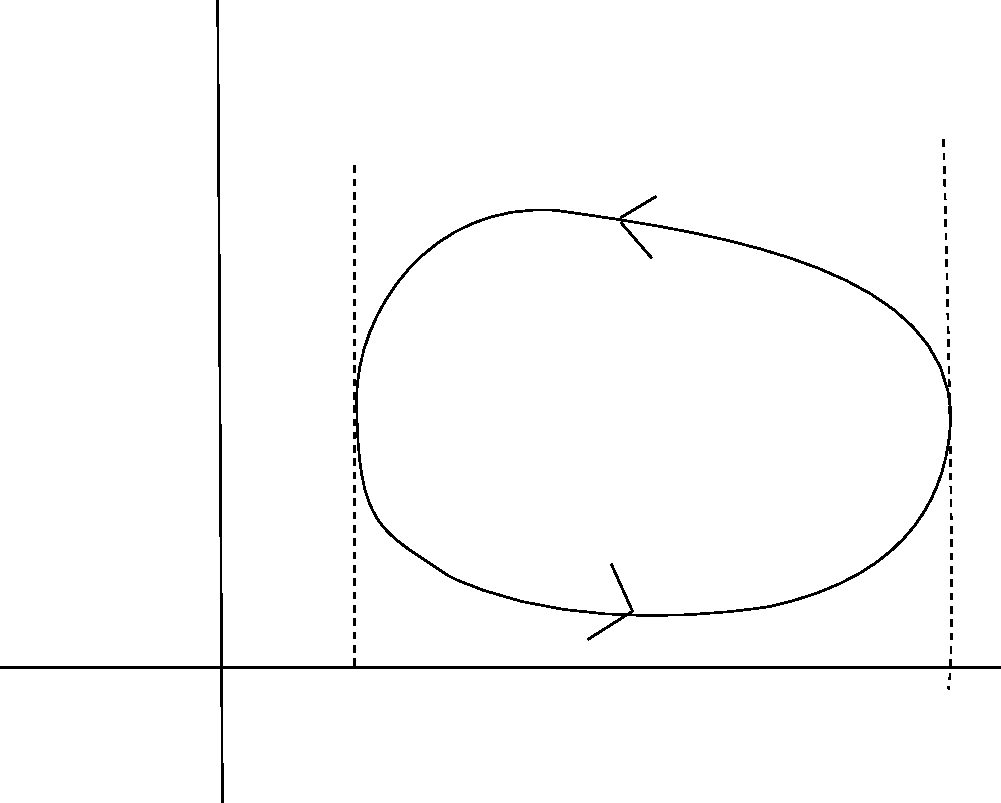
\includegraphics[width=3in]{Curve2.pdf}
\end{center}
Using the two points where the vertical tangents are located, we can split the curve into a top half and a bottom half. Clearly, the area bounded by the curve is equal to the area under the top half of the curve, minus the area under the bottom half.

Without loss of generality, suppose that our curve is parametrized by $F(t)=(x(t),y(t))$, for $t\in [t_0,t_2]$, such that $F(t_0)$ is the point on the curve corresponding to the vertical tangent on the left, and $t_1\in(t_0,t_2)$ is such that $F(t_1)$ is the point on the curve where the vertical tangent on the right occurs.

Since the curve is positively oriented, the interval $[t_0,t_1]$ gives the bottom half of the curve. Notice that $x'(t)>0$ for this half, since we're moving to the right ($x$ is increasing), and by assumption, $y(t)>0$ for all $t\in [t_0,t_2]$. The area under the bottom half of the curve is therefore
\[
A_{\text{bottom}} = \int_{t_0}^{t_1}y(t)x'(t)\,dt.
\]
Now, the top half of the curve is traced out for $t\in [t_1,t_2]$, but note that due to the orientation, we're travelling right to left, and thus $x'(t)<0$ on the top half. To get the area under the top half of the curve, we need to switch the sign to compensate:
\[
A_{\text{top}} = \int_{t_1}^{t_2}y(t)(-x'(t))\,dt = -\int_{t_1}^{t_2}y(t)x'(t)\,dt.
\]
The area enclosed by the curve is therefore:
\[
A  = A_{\text{top}}-A_{\text{bottom}}\\
=-\int_{t_1}^{t_2}y(t)x'(t)\,dt - \int_{t_0}^{t_1}y(t)x'(t)\,dt = -\int_{t_0}^{t_2}y(t)x'(t)\,dt,
\]
as claimed. For more complicated curves with more than two vertical tangents, we have to break the curve into a larger number of pieces, but the same type of argument will show that the area formula still works.
\section{Area in polar coordinates}
A polar curve is given by an equation of the form $r=f(\theta)$ in polar coordinates. This is a special case of a parametric curve, since the polar coordinate transformation gives us
\begin{align*}
 x &= r\cos\theta = f(\theta)\cos\theta\\
 y &= r\sin\theta = f(\theta)\sin\theta.
\end{align*}
The problem of arc length is the same for polar curves, and has the same difficulties (as far as being careful not to count points more than once). The arc length formula is simply the parametric arc length formula for the above parametrization, with simplifications. Since it's dealt with adequately in the textbook, we won't repeat that discussion here. Instead, we want to look at area. At first, one might expect that area is handled the same as arc length: since polar curves are parametric curves, and $\di A = -\int_\alpha^\beta y(\theta)x'(\theta)\,d\theta$, we need only substitute and compute the area. However, a few examples should convince you that this area formula is not well-adapted to polar curves. Fortunately, we have the formula
\[
 A = \int_\alpha^\beta\frac{1}{2}f(\theta)^2\,d\theta
\]
for polar area, which is derived from the formula $A = \dfrac{1}{2}r^2\Delta\theta$ for the area of a wedge of angular width $\Delta\theta$ of a circle of radius $r$ via the usual Riemann sum type of argument. It should be clear that the two area formulas compute different areas, based on the geometry used in each formula: the parametric area formula is approximated by a sum of areas of rectangles, while the polar area formula is approximated by a sum of areas of circular wedges. The difference is illustrated in the following diagram:
\begin{center}
 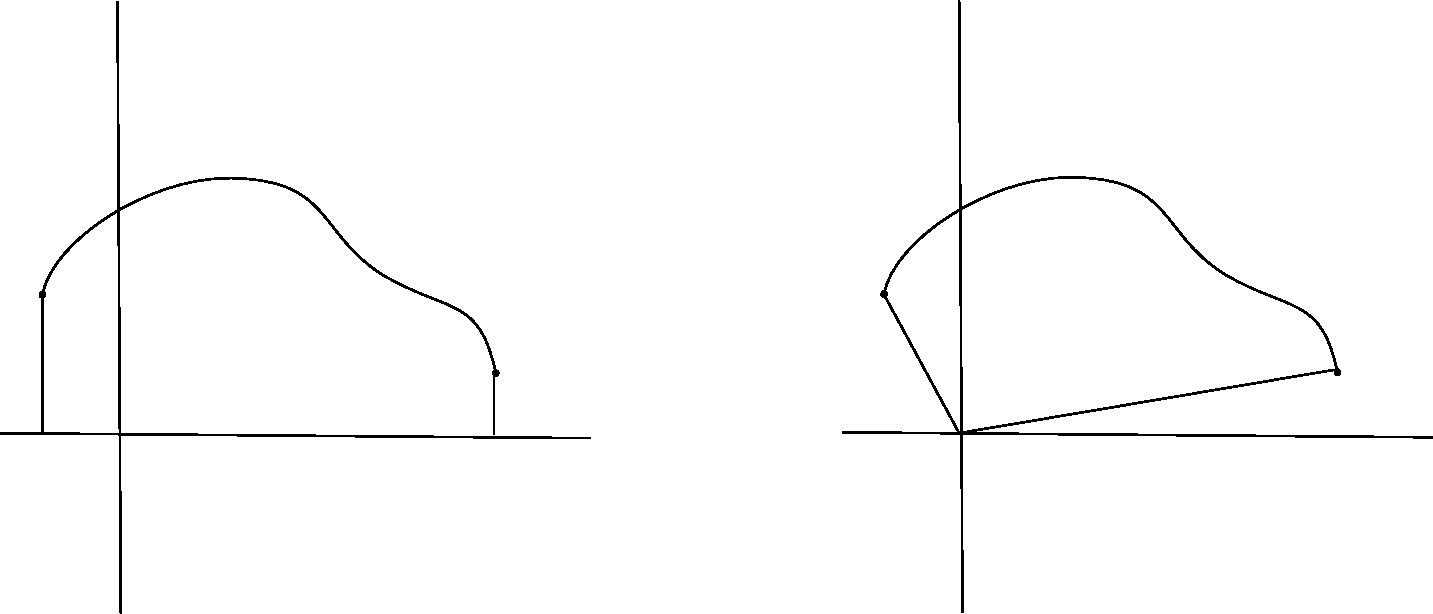
\includegraphics[width=4.5in]{polar_param.pdf}
\end{center}
However, for {\em closed} curves, we should expect that either area formula gives the same result, and indeed this is the case. Let $r=f(\theta)$, $\theta\in [\alpha,\beta]$ be any closed polar curve. (Caution: it need not be the case that $\beta = \alpha+2\pi$, although this is true for many examples. The condition that the curve be closed implies only that $x(\alpha)=x(\beta)$ and $y(\alpha)=y(\beta)$.)
Beginning with the parametric area formula, we have
\begin{align*}
A = -\int_\alpha^\beta y dx & = -\int_\alpha^\beta \left(f(\theta)f'(\theta)\sin\theta\cos\theta -f(\theta)^2\sin^2\theta \right)d\theta\\
&= \int_\alpha^\beta \left(\frac{1}{2}f(\theta)^2(1-\cos 2\theta)-\frac{1}{2}f(\theta)f'(\theta)\sin 2\theta\right)d\theta\\
&= \int_\alpha^\beta \frac{1}{2}f(\theta)^2d\theta -\int_\alpha^\beta \frac{d}{d\theta}\left(\frac{1}{4}f(\theta)^2\sin 2\theta\right)d\theta.
\end{align*}
But notice that $f(\theta)^2\sin 2\theta = 2f(\theta)^2\sin\theta\cos\theta = 2xy$, so the second integral in the last line above yields, via the fundamental theorem of calculus, $1/2(x(\alpha)y(\alpha)-x(\beta)y(\beta))$. But this is zero for a closed curve, and so we recover the polar area formula. Notice that if the curve is not closed, the second term in the last line will not necessarily vanish, and that it computes exactly the difference between the two areas. (Note also that, for example, $\di \frac{1}{2}x(\alpha)y(\alpha)$ is the area of one of the triangles that is missing on the right-hand side in the diagram above comparing the two area formulas.)

\end{document}
